\section{Correctness}
When we say that BPaxos is ``correct'', what do we mean? In this section, we'll
answer this question.

\subsection{Generalized Consensus on Logs}
In~\cite{lamport2005generalized}, Lamport introduces \defword{generalized
consensus}, a formalism that captures our intuition of what it means for a
consensus protocol to be correct. Generalized consensus is, as the name
implies, very general. It can be used to reason about consensus on logs, on
sets, on dependency graphs, you name it. Discussing generalized consensus in
full generality, requires us to define a new algebraic structure called a
\defword{command structure set}, or CStruct for short. These details get a bit
intense, and for our purposes, we don't need to discuss generalized consensus
in full generality. So, we'll skip the details and focus on two particular
instances of generalized consensus: generalized consensus on logs and
generalized consensus on traces.

\newcommand{\Cmd}{\Sigma}
\newcommand{\prefixof}{\sqsubseteq}
First up, \defword{generalized consensus on logs}. Protocols like MultiPaxos
and Raft implement consensus on logs. All replicas agree on a totally ordered
sequence of commands (called a log) that they all execute in exactly the same
order. Formally, let $\Cmd$ be a set of commands. A \defword{log} $x \in
\Cmd^*$ is simply a string of commands. We write $x \prefixof y$ to denote that
$x$ is a prefix of $y$, and we say that $z$ is an upper bound of $x$ and $y$ if
$x \prefixof z$ and $y \prefixof z$. A log consensus protocol (e.g.,
MultiPaxos, Raft) involves a set of clients that propose commands and a set of
learners that learn the state of the log over time. We say such a protocol
implements generalized consensus on logs if it satisfies the following
properties:
\begin{itemize}
  \item \textbf{Nontriviality:}
    At every point in time, the log $x$ learned by a learner can only contain
    commands proposed by a client.

  \item \textbf{Stability:}
    If a learner learns log $x$ at one point in time and log $y$ at a later
    point in time, then $x \prefixof y$. That is, a learner's log only grows
    over time.

  \item \textbf{Consistency:}
    For any two logs $x$ and $y$ learned by two different learners, there
    exists some upper bound of $x$ and $y$. That is, at any point in time two
    logs may not necessarily be equal, but they can be extended to be equal.

  \item \textbf{Liveness:}
    If a command is proposed, it eventually appears in a learned log.
\end{itemize}

Note that consistency allows two learners to have different logs so long as the
two logs can be extended to be equal. For example, logs $ab$ and $abcd$ are not
equal, but we can extend $ab$ to be equal to $abcd$. On the other hand, logs
$ab$ and $ba$ are not equal and \emph{cannot} be extended to be equal. In
effect, consistency forces all replicas to execute exactly the same commands in
the same order, while also allowing certain replicas to lag behind.

\subsection{Generalized Consensus on Traces}
\newcommand{\conflict}{\sim}
Next up, \defword{generalized consensus on traces}. Protocols like EPaxos,
BPaxos, Caesar, Generalized Paxos, and CURP implement consensus on traces.
Instead of agreeing on a totally ordered sequence of commands, replicas agree
on a partially ordered sequence of commands in which non-conflicting commands
can be executed in any order.

We formalize traces as \defword{Mazurkiewicz
traces}~\cite{mazurkiewicz1986trace}. Again consider a set $\Cmd$ of commands.
Also consider a symmetric conflict relation $\conflict$ over $\Cmd$. We say two
commands $a, b \in \Cmd$ conflict if $a \conflict b$. Consider two strings $x,
y \in \Cmd^*$. We say $x \approx y$ if there exists $u, v \in \Sigma^*$ and
non-conflicting commands $a, b \in \Sigma$ such that $x = uabv$ and $y=ubav$.
That is, $x \approx y$ if $y$ can be derived from $x$ by swapping a single pair
of adjacent non-conflicting commands. Let $\equiv$ be the symmetric,
transitive, reflexive closure of $\approx$. We say two strings are equivalent
if $x \equiv y$. Let $[x]$ be the equivalence class of string $x$ under
$\equiv$. We call $[x]$ a Mazurkiewicz trace. The set of all Mazurkiewicz
traces is the quotient $\Cmd/\equiv$ which is equal to $\setst{[x]}{x \in
\Sigma^*}$.

More informally, a Mazurkiewicz trace is a string of commands, except that we
are allowed to repeatedly replace adjacent non-conflicting commands. For
example, letting $\Cmd = \set{a, b, c, d}$ with $a \conflict b$, $a \conflict
c$, and $a \conflict d$, we have
\[
  abcd \approx abdc \approx adbc \approx adcb
\]
so $abcd$, $abdc$, $adbc$, and $adcb$ are all equivalent. They all represent
the same Mazurkiewicz trace. That is,
\[
  [abcd] = [abdc] = [adbc] = [adcb]
\]

Note that Mazurkiewicz traces appear in a lot of areas of computer science,
though often not under the same name. For example, the theory of database
serializability uses identical definitions to describe things like transaction
histories, conflicting reads and writes, and equivalent serial orders.  Also
note that Lamport calls Mazurkiewicz traces command
histories~\cite{lamport2005generalized}.

Another important bit of theory is that Mazurkiewicz traces are isomorphic to
dependency graphs. A \defword{dependency graph} $G = (V, E, \phi)$ is an
acyclic directed graph $(V, E)$ with a function $\phi: V \to \Cmd$ that labels
each vertex with a command. The dependency graph corresponding to Mazurkiewicz
trace $[a_1 a_2 \ldots a_n]$ has $n$ vertices labelled $a_1, \ldots, a_n$. The
vertex labelled $a_i$ has an edge to every vertex labelled $a_j$ where $j < i$
and $a_i \conflict a_j$. Conversely, The Mazurkiewicz trace corresponding to a
dependency graph can be formed by topologically sorting the graph. Considering
the example from above, the trace $[abca]$ has the following dependency graph:
\begin{center}
  \tikzstyle{vert}=[draw, thick]
  \tikzstyle{dep}=[-latex, thick]
  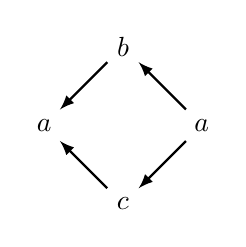
\begin{tikzpicture}
    \node (a0) at (0, 0) {$a$};
    \node (b) at (1, 1) {$b$};
    \node (c) at (1, -1) {$c$};
    \node (a1) at (2, 0) {$a$};
    \draw[dep] (b) to (a0);
    \draw[dep] (c) to (a0);
    \draw[dep] (a1) to (b);
    \draw[dep] (a1) to (c);
  \end{tikzpicture}
\end{center}
Topologically sorting the graph, we get strings $abca$ or $acba$, which
are equivalent.

Now that we've formalized traces and dependency graphs, we return to
generalized consensus. We write $[x] \prefixof [y]$ to denote that trace $[x]$
is a prefix of trace $[y]$ (that is, there exists some $z \in \Cmd^*$ such that
$[xz] = [y]$).  We say $[z]$ is an upper bound of $[x]$ and $[y]$ if $[x]
\prefixof [z]$ and $[y] \prefixof [z]$. A trace consensus protocol (e.g.,
EPaxos, BPaxos, Generalized Paxos) involves a set of clients that propose
commands and a set of learners that learn the state of the trace over time. We
say such a protocol implements generalized consensus on traces (or command
histories) if it satisfies the following properties:
\begin{itemize}
  \item \textbf{Nontriviality:}
    At every point in time, the trace $[x]$ learned by a learner can only
    contain commands proposed by a client.

  \item \textbf{Stability:}
    If a learner learns trace $[x]$ at one point in time and trace $[y]$ at a
    later point in time, then $[x] \prefixof [y]$. That is, a learner's trace
    only grows over time.

  \item \textbf{Consistency:}
    For any two traces $[x]$ and $[y]$ learned by two different learners, there
    exists some upper bound of $[x]$ and $[y]$. That is, at any point in time
    two traces may not necessarily be equal, but they can be extended to be
    equal.

  \item \textbf{Liveness:}
    If a command is proposed, it eventually appears in a learned trace.
\end{itemize}

Note that the correctness criteria of generalized consensus on logs and the
correctness criteria of generalized consensus on traces are more or less the
same.
%
Moreover, if we write $x \prefixof y$ to denote that dependency graph $x$ is a
prefix of dependency graph $y$, and if we say $z$ is an upper bound of $x$ and
$y$ if $x \prefixof z$ and $y \prefixof z$, then we can define generalized
consensus on dependency graphs exactly as we did for traces. Generalized
consensus on traces and generalized consensus on dependency graphs are exactly
the same thing.

\subsection{EPaxos Correctness Criteria}
Generalized consensus has a lot of attractive qualities. It's formal but
intuitive. It's general. It's been around for a while. Ideally, researchers
would invent new consensus protocols that implement generalized consensus and
not bother inventing new correctness criteria for every new protocol. And in
fact, since Lamport introduced generalized consensus, this has largely been the
case. Generalized Paxos uses generalized consensus. GPaxos uses generalized
consensus. BPaxos uses generalized consensus. So does Caesar.

However, EPaxos notably does not use it. Instead, EPaxos implements a new set
of correctness criteria with definitions of nontrivialty, stability,
consistency, execution consistency, execution linearizability, and liveness.
Nontriviality, stability, and liveness are essentially the same as in
generalized consensus. Execution linearizability is just linearizability, a
nice property to add. Consistency is an implementation detail of EPaxos. The
most interesting criterion is execution consistency which is defined as ``If
two interfering commands $\gamma$ and $\delta$ are successfully committed (by
any replicas) they will be executed in the same order by every replica''.

Execution consistency replaces generalized consensus' definition of
consistency. The new definition, unfortunately, has a couple of flaws.
\begin{itemize}
  \item
    First, commands can be executed multiple times, but the definition of
    execution consistency does not disambiguate between repeated commands.
    For example, if a replica executes $\gamma$ then $\delta$ then $\gamma$
    again, did it execute $\gamma$ before $\delta$ or after?
  \item
    Second, execution consistency is defined with a sense of liveness in it.
    It says commands ``will be executed''. It's preferable to separate out
    safety properties from liveness properties.
  \item
    Third, the distinction between committing a command and executing a command
    is an implementation detail of EPaxos. Ideally, the correctness criterion
    would not rely on this implementation detail.
  \item
    Finally, it's unclear how EPaxos' correctness criteria relate to those of
    generalized consensus. Are the two equivalent? If not, how do they differ?
\end{itemize}

However, these flaws are largely minor and pedantic.  EPaxos' correctness
criteria have the major advantage of simplicity.  The new definitions are
\emph{much} simpler to digest than a full blown description of generalized
consensus. The EPaxos paper doesn't have to define traces or dependency graphs,
it doesn't have to discuss prefixing or upper bounds, and it doesn't have to
introduce generalized consensus at all. The new criteria get to the heart of
the matter: conflicting commands should be executed in the same order on all
replicas.

\subsection{Reconciling Generalized Consensus and EPaxos}
In this section, we show that EPaxos' correctness criteria are easy to
formalize and that they are in fact equivalent to those of generalized
consensus on traces. This result lets us think about the correctness of EPaxos
and BPaxos either through the lens of forming dependency graphs or through the
lens of ensuring that conflicting commands are ordered the same across all
replicas.

First, we formalize the notion that one replica executes command $a$ before
command $b$. EPaxos and BPaxos replicas sequentially execute commands. These
commands form a trace $a_1, \ldots, a_n \in \Cmd^*$. The trace may contain
duplicates but fortunately, every command is chosen in a unique instance. Thus,
we can essentially think of commands as unique, where command $a$ chosen in
instance $I$ is different from command $a$ chosen in instance $J$.

Let $x \in \Cmd^*$ be such a trace. Let $a$ and $b$ be conflicting commands. We
say $a$ happens before $b$ in $x$, denoted $a < b$ in $x$, if one of the
following things is true:
\begin{itemize}
  \item
    $a, b \in x$ and $a$ precedes $b$ in $x$. Note that if $a$ and $b$ did not
    conflict, the notion of $a$ preceding $b$ would be ill-defined since a
    trace can re-order non-conflicting commands.

  \item
    $a \in x$ and $b \notin x$.
\end{itemize}
We say $a$ could happen before $b$ in $x$, denoted $x <_? b$ in $x$, if $a < b$
in $x$ or $a, b \notin x$.

Now, we can define EPaxos' correctness criteria the same as generalized
consensus on traces, except we'll define consistency as follows. For any two
traces $x$ and $y$ executed by two replicas, and for any two conflicting
commands $a$ and $b$, if $a < b$ in $x$ then $a <_? b$ in $y$.

TODO: Differentiating between $<$ and $<_?$ is a bit subtle. Work that out.

TODO: Prove that EPaxos consistency implies Generalized Consensus consistency.
- Long case analysis.

TODO: Prove that Generalized Consensus consistency implies EPaxos consistency.
- Prove that if $a < b$ in $x$, then $a < b$ in all prefixes of $x$.
- Case analysis.

% Well, defining the
% correctness of a state machine replication protocol like BPaxos turns out to be
% more complex that it may seem.
%
% Generalized
% Paxos~\cite{lamport2005generalized} formalizes \defword{generalized consensus}
% quite nicely, but it's pretty complicated. EPaxos defines its own form of
% correctness, but it's a tiny bit informal. Caesar~\cite{arun2017speeding}
% defines correctness using generalized consensus, but again, this is a little
% too complicated.
%
% Ideally, we'd like to define a very intuitive correctness criterion and prove
% that it is equivalent to generalized consensus. Here's an attempt at that.
%
% Let $\Sigma$ be a set of commands. Let $\Sigma!$ be the strings over $\Sigma$
% with no repeated commands. Let $x = x_1 \ldots x_n \in \Sigma!$. We say $a < b$
% in $x$ if (a) $a$ and $b$ both appear in $x$ and $a$ precedes $x$, or (b) $a$
% appears in $x$ but not $b$, or (c) neither appears in $x$. Consider two strings
% $x, y$ such that $a < b$ in $x$ if and only if $a < b$ in $y$. We want to prove
% that $x$ and $y$ are compatible. That is, there exists strings $w_x$ and $w_y$
% such that $x w_x \equiv y w_y$. If this is true, then the informal statement
% ``replicas execute conflicting commands in the same order'' is enough to
% maintain generalized consensus.
%
% The proof is likely going to be tricky. Reasoning about the equivalence of
% commands is always tricky. I think $w_x = y - x$ and $w_y = x - y$, but we'll
% have to see.
%
% Proof idea:
% In the Generalized Paxos paper, they say two histories are equivalent if they
% are permutations that preserve conflicting command ordering. If this is true,
% then I think we can prove our theorem easily. Append $(y-x) to x$ and $(x-y) to
% y$. They are permutations. Then, look at a conflicting pair of commands $a, b$
% in $x(y-x)$. Do a case analysis on where $a$ and $b$ appear. $a,b$ both in $x$;
% $a$ in $x$, $b$ in $(y-x)$, $a,b$ both in $(y-x)$. In all cases, we'll see that
Defining % $y(x-y)$ has them in the same order. Thus, the two strings are equivalent.
